\chapter{Musik}
I dette afsnit vil der blive analyseret 5 forskellige musiksekvenser, vi selv har valgt. \\
Der vil være 4 forskellige grafer for hver musiksekvens.\\ \\
Den først viser signalet som funktion af tiden - her befinder signalet sig i tidsdomænet. \\
De 2 næste viser signalet magnitude som funktion af frekvens i Hz. Den sidste af disse viser signalet på en logaritmisk x-akse. \\
Den sidste graf viser fasen som funktion af frekvens i Hz. De sidste 3 befinder sig frekvens-domænet, da vi har lavet en DFT af signalet.   

\section{Cool music}

\begin{figure}[H]
	\centering
	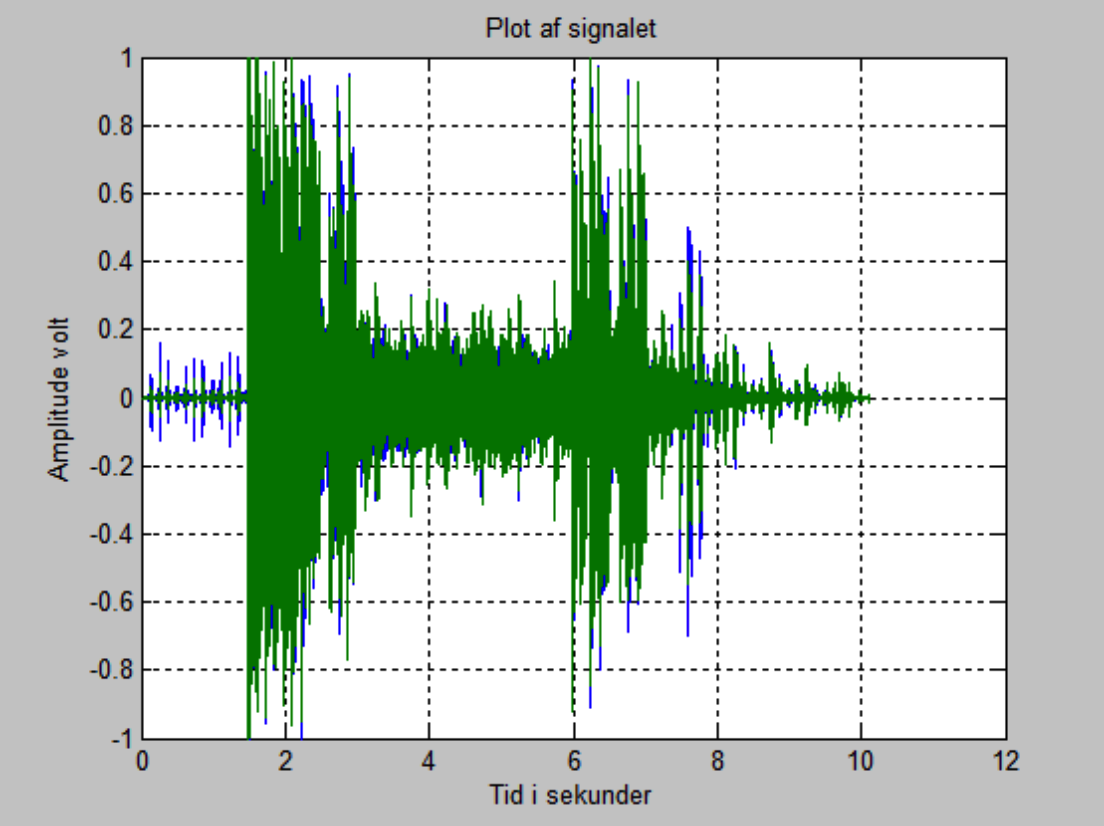
\includegraphics[width=0.8\textwidth]{Figurer/Snip20151001_3}
	\caption{\textit{Cool music} - Signal som funktion af tiden i sekunder}
\end{figure}

Det er et stykke elektronisk musik på 10 sekunder. Vi kan se, at der er nogle store amplituder flere steder i musiksekvensen. I det første område med store amplituder, er der en tromme, der går lidt mere amok i forhold til resten af sekvensen. Den sidste halvdel med store amplituder bliver der scratchet og så dør sekvensen ud.

\begin{figure}[H]
	\centering
	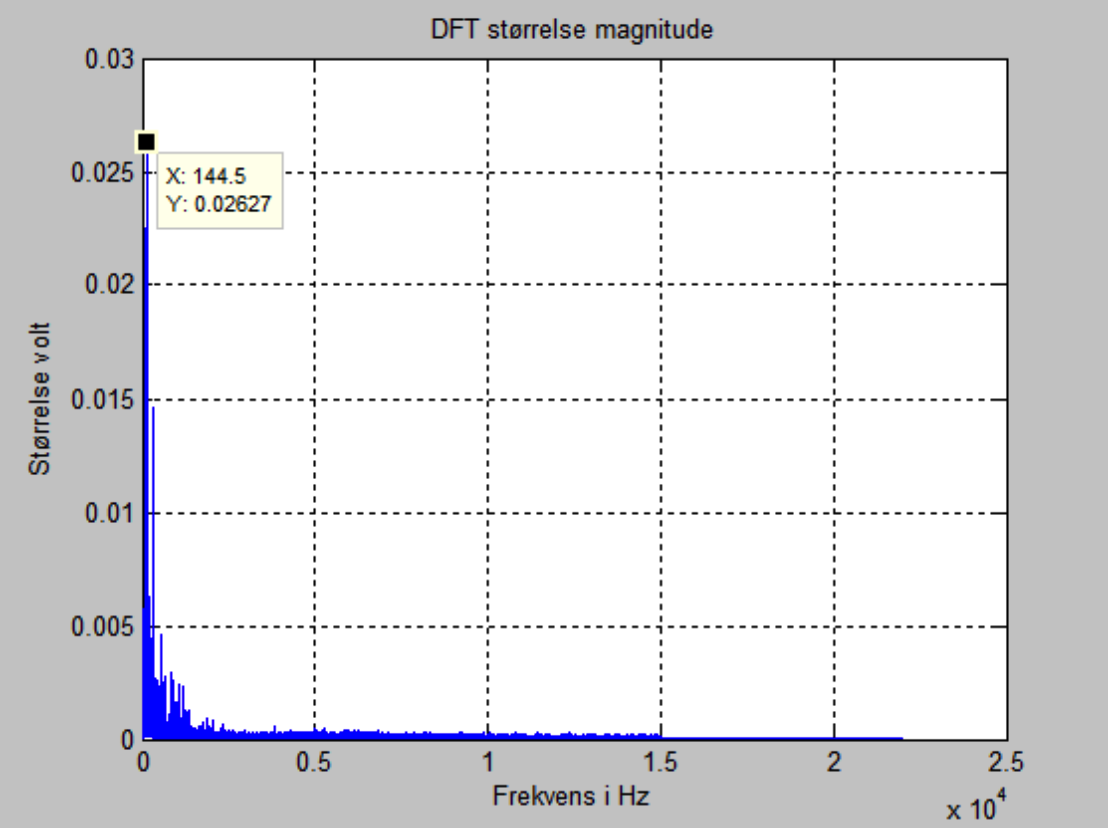
\includegraphics[width=0.8\textwidth]{Figurer/Snip20151001_7}
	\caption{\textit{Cool music} - Signalets magnitude som funktion af frekvens i Hz}
\end{figure}

Fra 0 til 500 Hz er der meget energi i musiksekvensen - dette kan vi se, da der er en meget høj volt (ca. 0,005-0,025) i dette område i forhold til resten af sekvensen, som ligger imellem 0-0,005. Den største amplitude ligger ved 144,5 Hz.      

\begin{figure}[H]
	\centering
	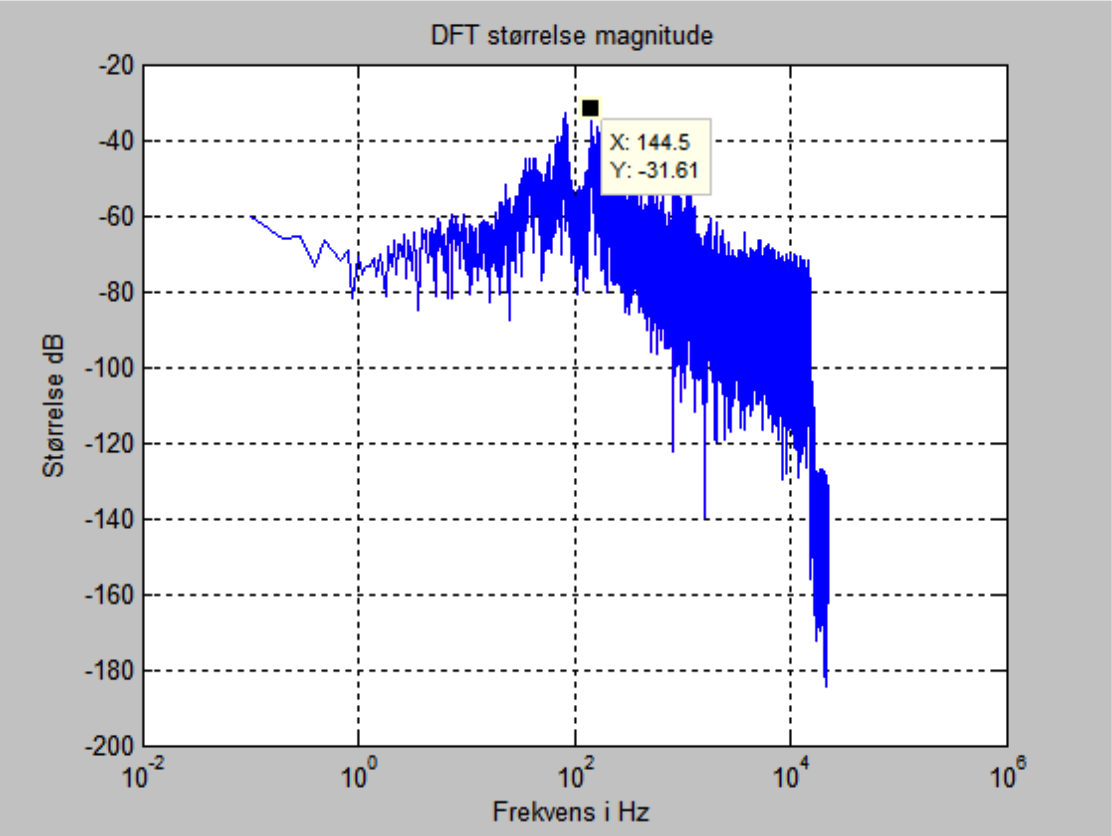
\includegraphics[width=0.8\textwidth]{Figurer/Snip20151001_8}
	\caption{\textit{Cool music} - Signalets magnitude som funktion af frekvens i Hz. Logaritmisk x-akse}
\end{figure}  

Vi har valgt, at plotte musiksekvensen med en logaritmisk x-aksen, da det på den måde bliver mere tydeligt, hvordan signalet opfører sig. Y-aksen bliver et udtryk af størrelse målt i dB. \\
Vi kan se, at den største amplitude også her ligger ved 144,5 Hz. Denne frekvens ligger tæt på D3 tonen, som er på 146,832 Hz.      


\begin{figure}[H]
	\centering
	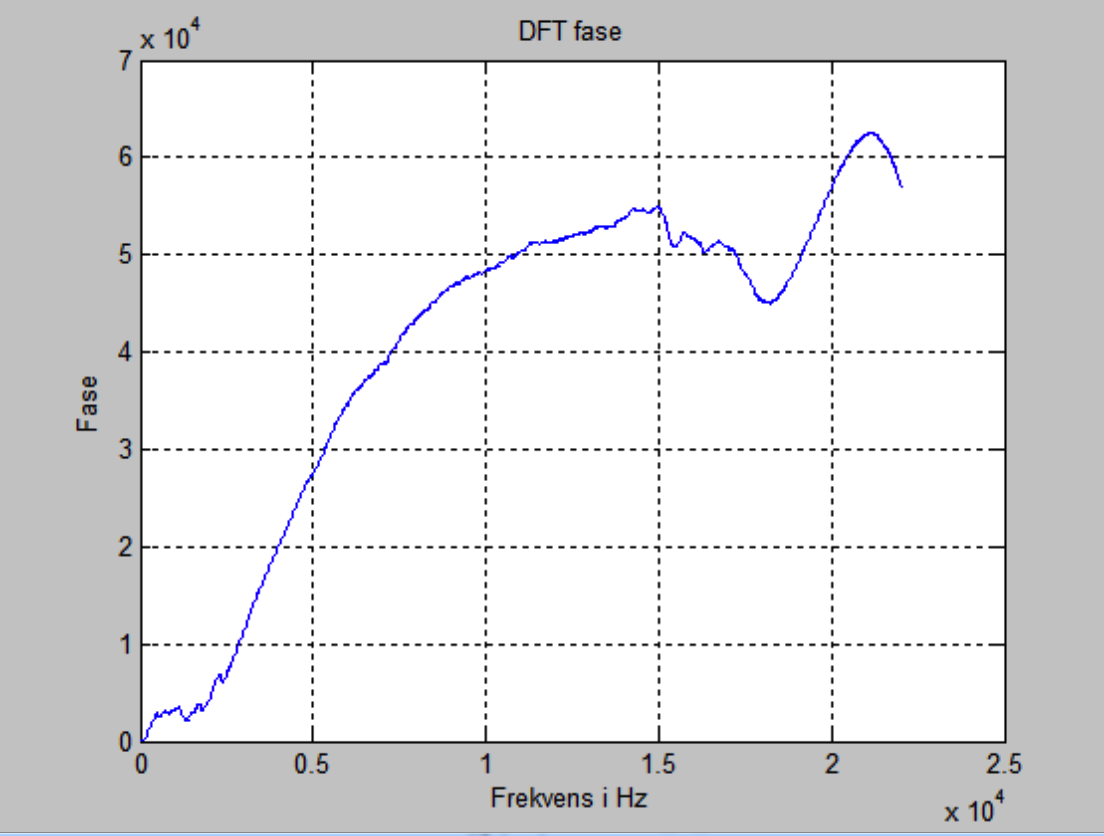
\includegraphics[width=0.8\textwidth]{Figurer/Snip20151001_6}
	\caption{\textit{Cool music} - Signalets fase som funktion af frekvens i Hz}
\end{figure} 

Der er fasedrejninger fra 15000 Hz til 22000 Hz. 

\section{Drum roll}
 
\begin{figure}[H]
	\centering
	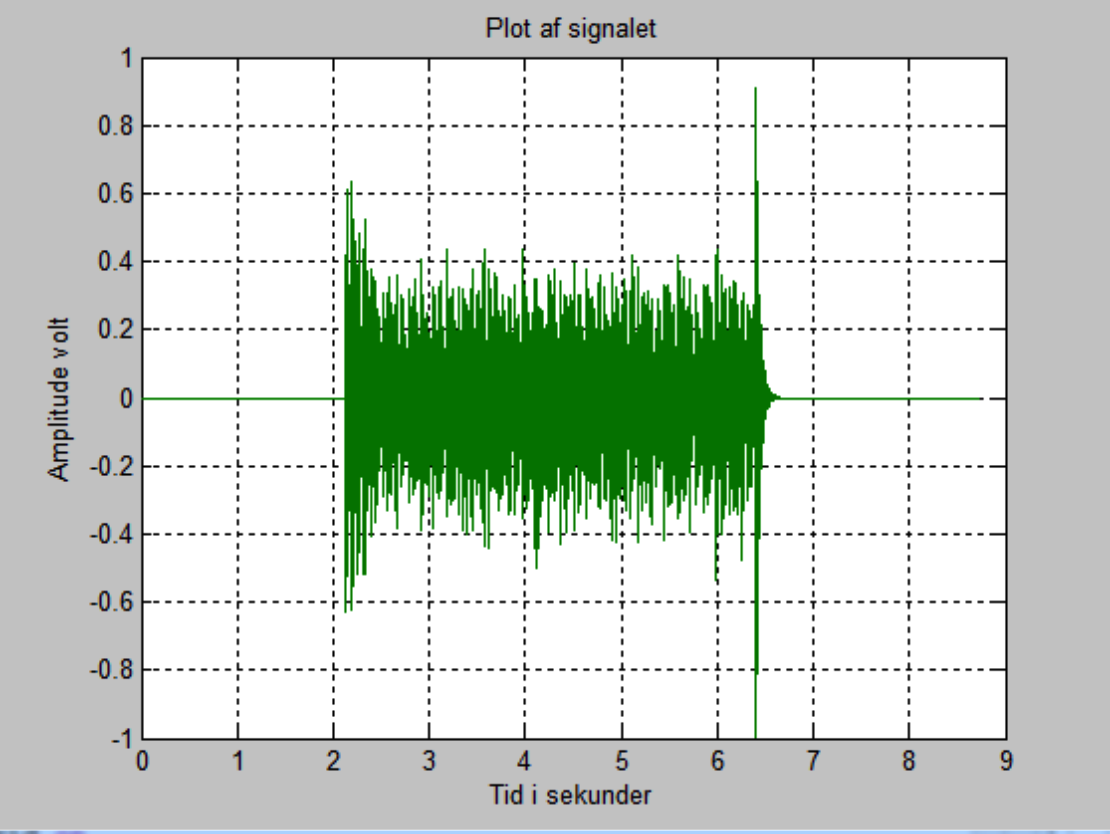
\includegraphics[width=0.8\textwidth]{Figurer/Snip20151001_9}
	\caption{\textit{Drum roll} - Signal som funktion af tiden i sekunder}
\end{figure}

Hvis man ser bort fra 2,5 sekund og de sidste 3 sekunder, ses det at amplitudespekteret ikke varier ret meget, hvilket vil sige, at det er meget monotont. Det stemmer meget overens med, når man lytter til musiksekvensen. Der er 2 pauser i sekvensen - i starten og tilsidst. Det kan vi se ved, at der ingen amplitude er - den ligger bare konstant på 0. Lige når trommens lyd begynder er der en større aktivitet end i det monotone afsnit. Ved 6,3 sekunder befinder den største amplitude sig - her bliver der i musiksekvensen muligvis slået ekstra meget i trommen.  

\begin{figure}[H]
	\centering
	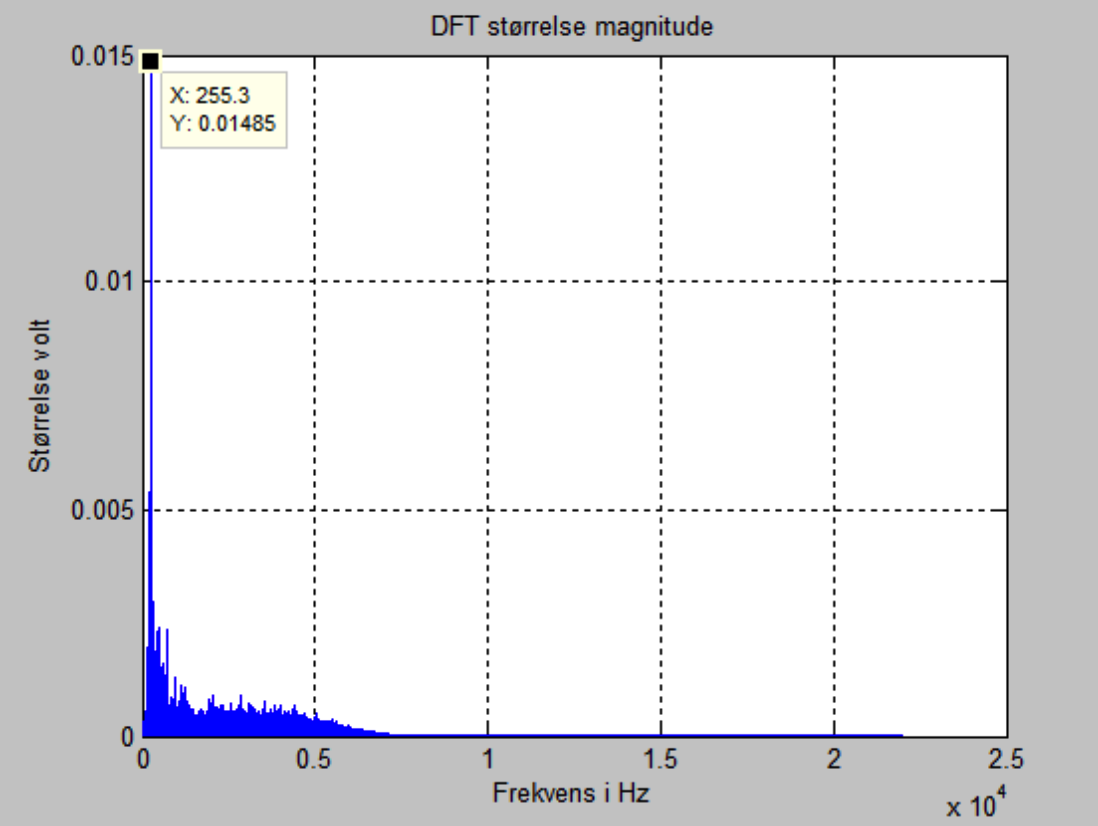
\includegraphics[width=0.8\textwidth]{Figurer/Snip20151001_14}
	\caption{\textit{Drum roll} - Signalets magnitude som funktion af frekvens i Hz}
\end{figure}

 Den største amplitude ligger ved 255,3 Hz. Frekvenserne efter ca. 500 Hz har en markant lavere energi.

\begin{figure}[H]
	\centering
	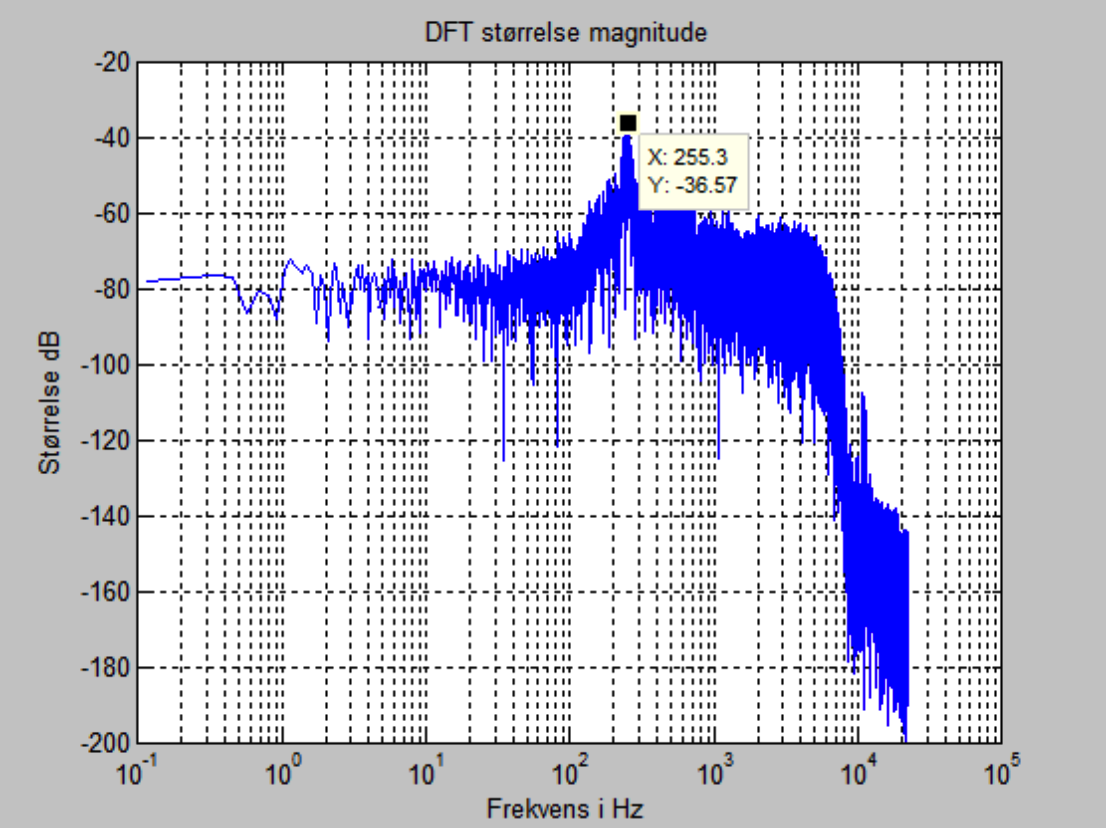
\includegraphics[width=0.8\textwidth]{Figurer/Snip20151001_12}
	\caption{\textit{Drum roll} - Signalets magnitude som funktion af frekvens i Hz. Logaritmisk x-akse}
\end{figure} 

Vi har valgt, at plotte musiksekvensen med en logaritmisk x-aksen, da det på den måde bliver mere tydeligt, hvordan signalet opfører sig. Y-aksen bliver et udtryk af størrelse målt i dB. \\
Vi kan se, at den største amplitude også her ligger ved 255,3 Hz. Denne frekvens ligger forholdsvis tæt på C4 tonen, som er på 262 Hz.   

\begin{figure}[H]
	\centering
	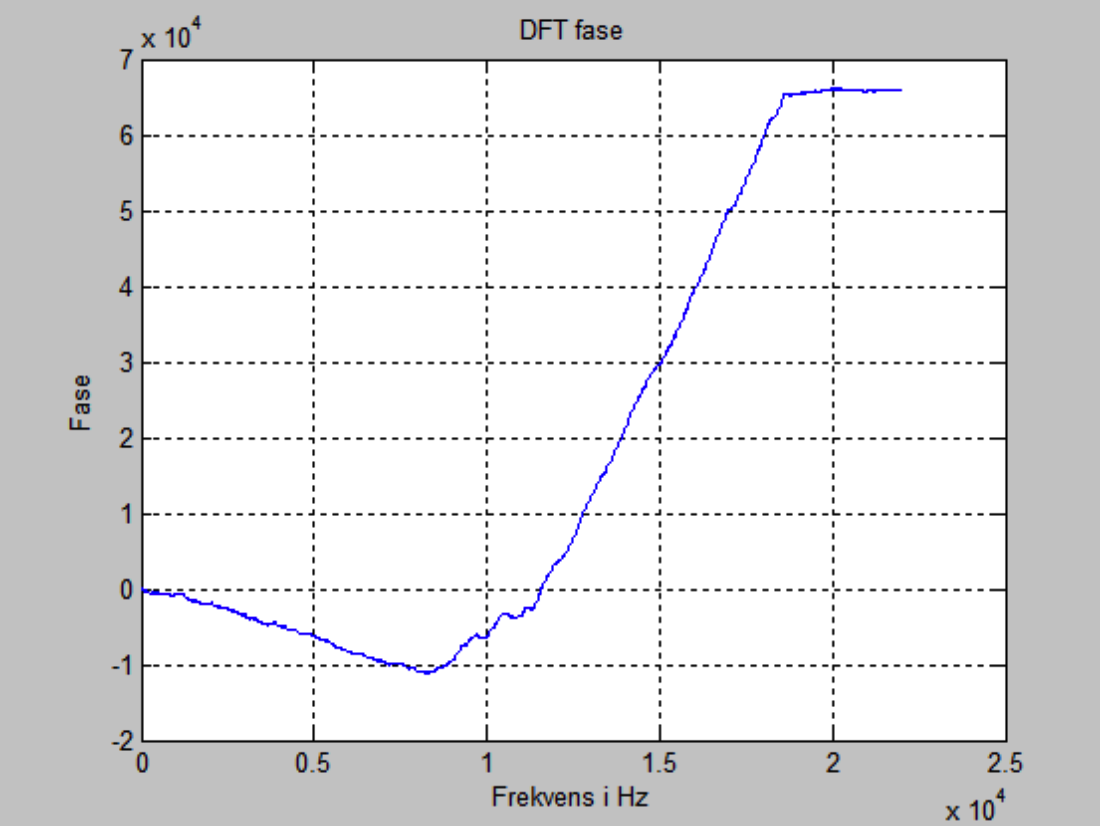
\includegraphics[width=0.8\textwidth]{Figurer/Snip20151001_15}
	\caption{\textit{Drum roll} - Signalets fase som funktion af frekvens i Hz}
\end{figure} 

Der ses en fasedrejning ved ca. 8000 Hz, hvorefter fasen stiger kontinuerligt til ca. 18000 Hz.

\section{Straight outta Compton}

\begin{figure}[H]
	\centering
	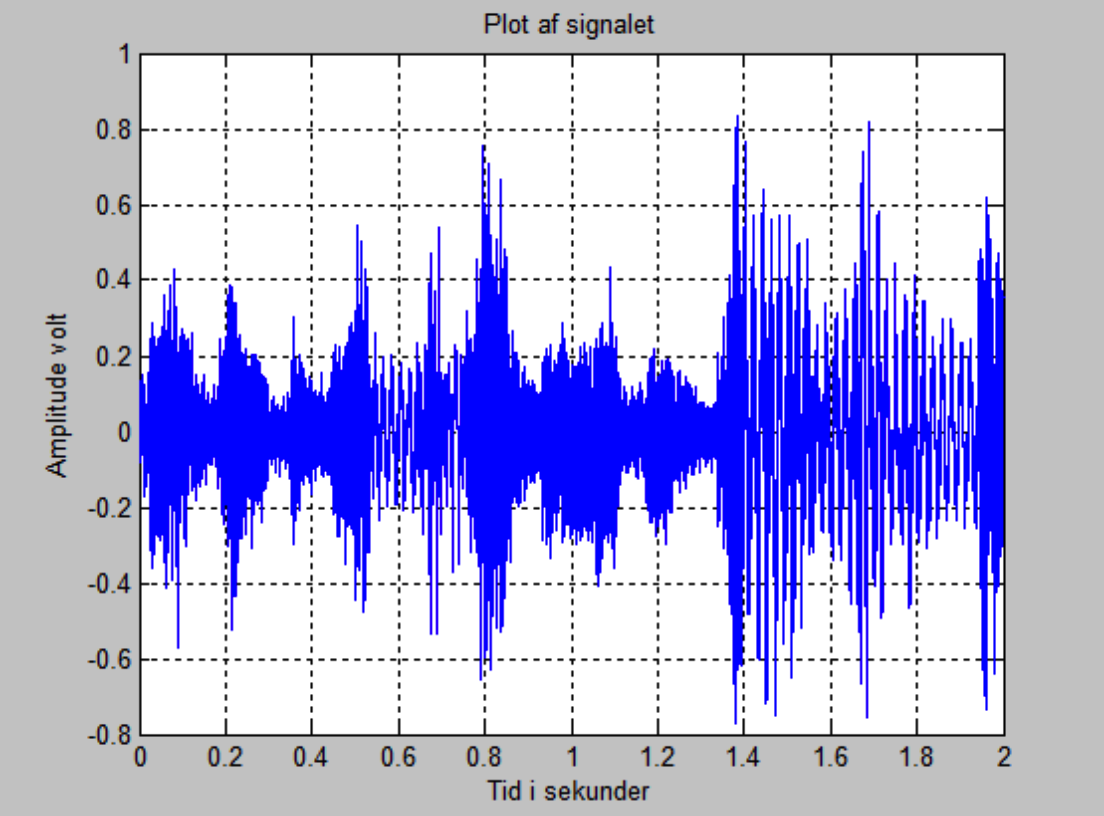
\includegraphics[width=0.8\textwidth]{Figurer/Snip20151001_16}
	\caption{\textit{Straight outta Compton} - Signal som funktion af tiden i sekunder}
\end{figure}

Vi arbejder her med gruppen N.W.A. og deres nummer 'Straight outta Compton', hvor vi har valgt, at kigge nærmere på en lydsekvens fra 92 sekunder inde i sangen. Den lydsekvens vi har kigget på strækker sig over 2 sekunder. Lige som med 'Uptown funk' i musikstykke 4, så ses det, at denne lydsekvens ligeledes benytter et bredt amplitudespekter. Specielt fra 1,35 sekunder stiger amplituden markant, hvorefter den svinger voldsomt resten af lydsekvensen.

\begin{figure}[H]
	\centering
	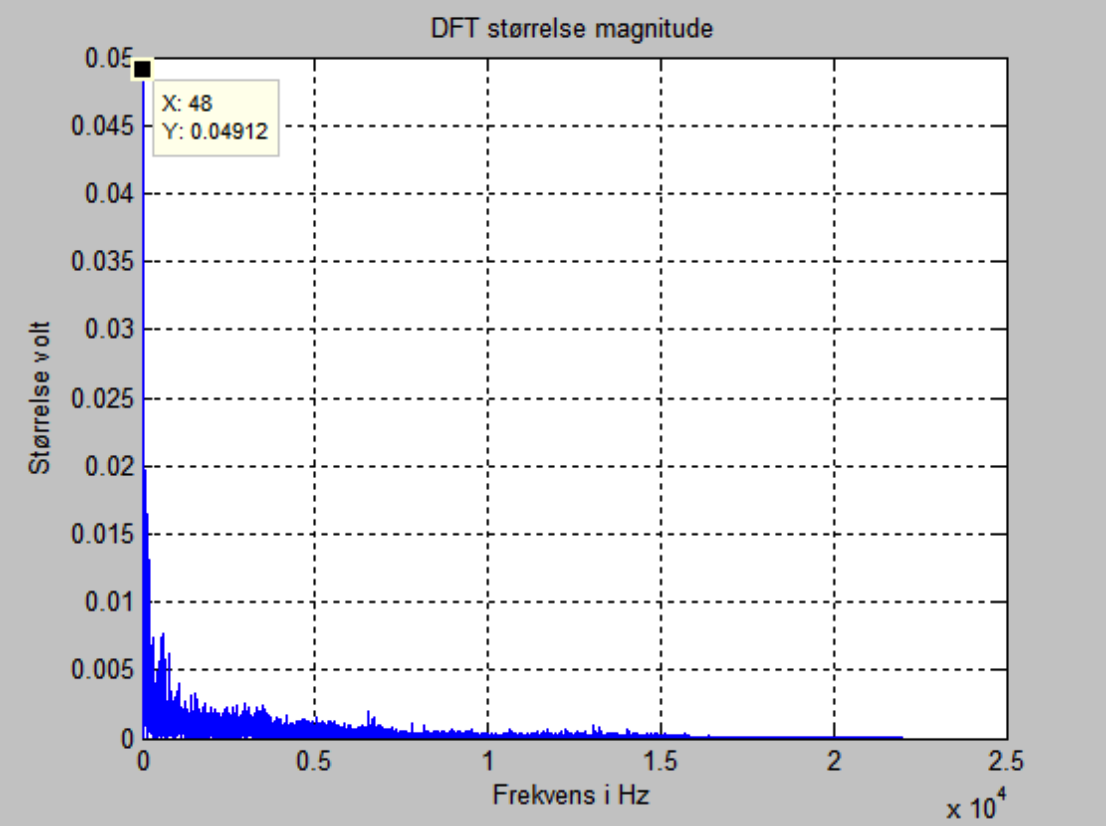
\includegraphics[width=0.8\textwidth]{Figurer/Snip20151001_17}
	\caption{\textit{Straight outta Compton} - Signalets magnitude som funktion af frekvens i Hz}
\end{figure}

\begin{figure}[H]
	\centering
	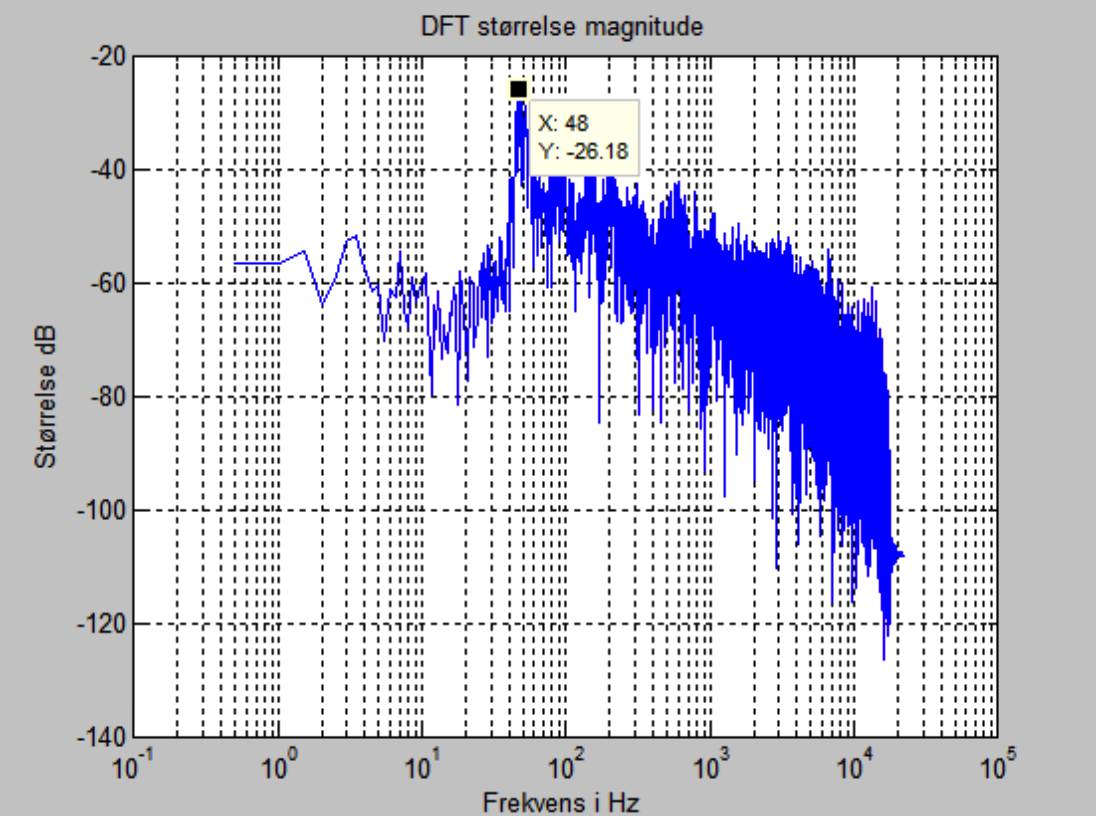
\includegraphics[width=0.8\textwidth]{Figurer/Snip20151001_18}
	\caption{\textit{Straight outta Compton} - Signalets magnitude som funktion af frekvens i Hz. Logaritmisk x-akse}
\end{figure} 

Den størst amplitude har en frekvens på 48 Hz. Det er betydelig lavere end de andre musiksekvenser, der er blevet analyseret. En god forklaring på dette er, at det er en rapsang. Rap er snak - så derfor er det lavfrekvens, der er mest tydelig i denne musiksekvens.  

\begin{figure}[H]
	\centering
	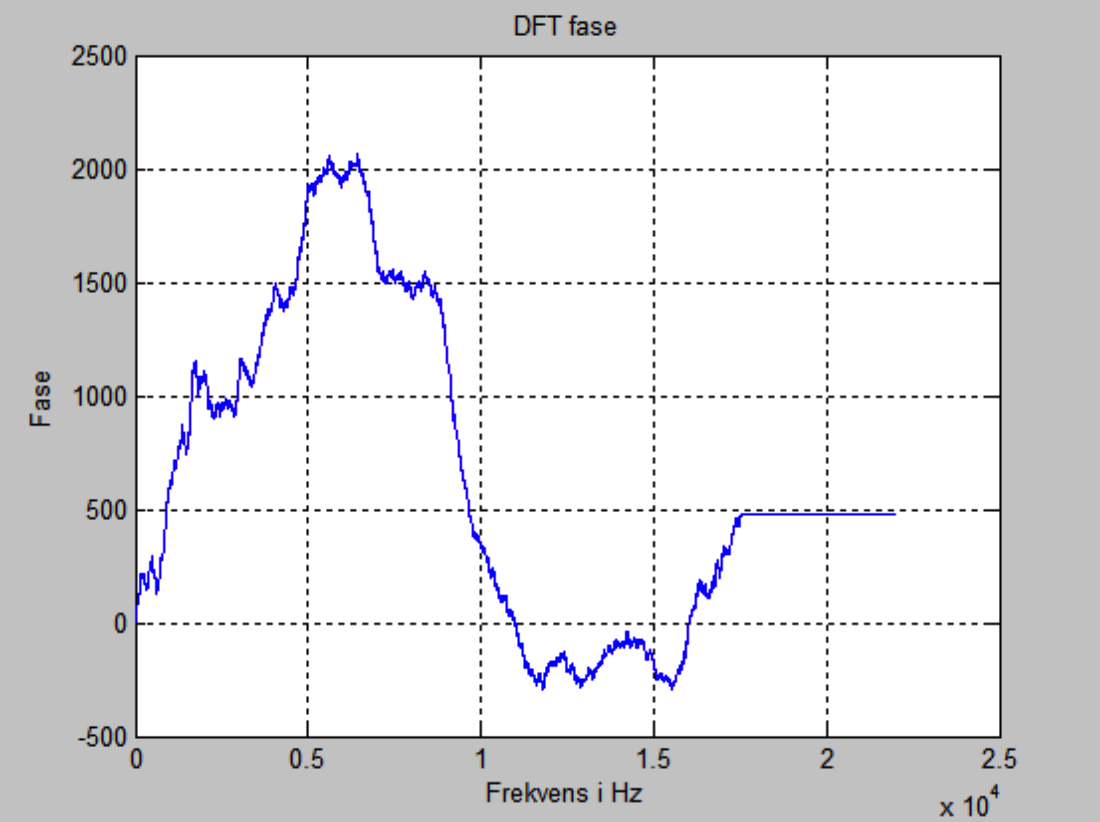
\includegraphics[width=0.8\textwidth]{Figurer/Snip20151001_19}
	\caption{\textit{Straight outta Compton} - Signalets fase som funktion af frekvens i Hz}
\end{figure} 













